\documentclass[a4paper,11pt]{book}

\usepackage[top=2cm,bottom=2cm,left=2cm,right=2cm]{geometry}
\usepackage[a-1b]{pdfx}
%\usepackage[pdftex]{graphicx} %per poter inserire le figure
\usepackage{graphicx}
%\usepackage[utf8]{inputenc}
\usepackage[T1]{fontenc}
\usepackage{amssymb,amsmath,amsthm,amsfonts}
\usepackage{xspace}
\usepackage{tabularx}
\usepackage{indentfirst}
\usepackage{subfigure}
\usepackage[small]{caption}
\usepackage{eucal}
\usepackage{eso-pic}
\usepackage{url}
\usepackage{booktabs}
\usepackage{afterpage}
\usepackage{parskip}
\usepackage{listings}
\usepackage{fancyhdr}
\usepackage{textcomp}
\usepackage{cite}
\usepackage{multirow}
\usepackage{setspace}
\pagestyle{fancy}
\usepackage[italian]{babel}
\usepackage{lipsum}


\usepackage{float}
\usepackage{listings}
%\usepackage[usenames]{color}
%\usepackage{natbib}
\usepackage{siunitx}
\usepackage[strict]{changepage}
\usepackage{physics}
\usepackage{wrapfig}
\usepackage{array}
\usepackage{color}
\usepackage{colortbl}
\usepackage{multirow}
\usepackage{enumitem}
%\usepackage{hyperref}
\usepackage{times}
%\usepackage{subfig}

\DeclareUnicodeCharacter{2009}{\,} 
\DeclareSIUnit\solarmass{M\ensuremath{_\odot}}
\newcommand{\smallsim}{\smallsym{\mathrel}{\sim}}

\makeatletter
\newcommand{\smallsym}[2]{#1{\mathpalette\make@small@sym{#2}}}
\newcommand{\make@small@sym}[2]{%
	\vcenter{\hbox{$\m@th\downgrade@style#1#2$}}%
}
\newcommand{\downgrade@style}[1]{%
	\ifx#1\displaystyle\scriptstyle\else
	\ifx#1\textstyle\scriptstyle\else
	\scriptscriptstyle
	\fi\fi
}

%Includes "References" in the table of contents
\usepackage[nottoc]{tocbibind}

%   Reduce the margin of the summary:
%\def\changemargin#1#2{\list{}{\rightmargin#2\leftmargin#1}\item[]}
%\let\endchangemargin=\endlist 

%   Generate the environment for the abstract:
%\newcommand\summaryname{Abstract}
%\newenvironment{Abstract}%
%    {\small\begin{center}%
%    \bfseries{\summaryname} \end{center}}

\includeonly{Capitoli/Capitolo_1/Capitolo_1,
			 Capitoli/Capitolo_2/Capitolo_2,
			 Capitoli/Capitolo_3/Capitolo_3,
			 Capitoli/Capitolo_4/Capitolo_4,
			 Capitoli/Conclusioni/Conclusioni}

\begin{document}
	
	\frontmatter
	\begin{titlepage}
		\vspace{5mm}
		\begin{figure}[hbtp]
			\centering
			
\includegraphics[scale=.13]{UNIPD.png}
		\end{figure}
		
		\vspace{5mm}
		
		\begin{center}
			{{\huge{\textsc{\bf UNIVERSIT\`A DEGLI STUDI DI PADOVA}}}\\}
			\vspace{5mm}
			{\Large{\bf Dipartimento di Fisica e Astronomia ``Galileo Galilei''}} \\
			\vspace{5mm}
			{\Large{\textsc{\bf Corso di Laurea in Fisica}}}\\
			\vspace{20mm}
			{\Large{\textsc{\bf Tesi di Laurea}}}\\
			\vspace{30mm}
			\begin{spacing}{3}
				{\LARGE \textbf{Ricerca di segnali gravitazionali dovuti alla coalescenza di sistemi binari di stelle di neutroni nella fase di post coalescenza}}\\
			\end{spacing}
			\vspace{8mm}
		\end{center}
		
		\vspace{20mm} %era 20
		
		\begin{spacing}{2}
			\begin{tabular}{ l  c  c c c  cc c c c c  l }
				{\Large{\bf Relatrice}} &&&&&&&&&&& {\Large{\bf Laureando}}\\
				{\Large{\bf Dott.ssa Claudia Lazzaro}} &&&&&&&&&&& {\Large{\bf Aidin Attar}}\\
				%{\Large{\bf Correlatore}}\\
				%{\Large{\bf Prof./Dr. Nome Cognome}}\\
			\end{tabular}
		\end{spacing}
		\vspace{15 mm} %era 15
		
		\begin{center}
			{\Large{\bf Anno Accademico 2020/2021}}
		\end{center}
	\end{titlepage}
	\clearpage{\pagestyle{empty}\cleardoublepage}
	
	
	
	%    \nocite{*}
	
	%    \setlength{\headheight}{14pt}
	\tableofcontents
	%    \listoffigures
	
	%    \begin{Abstract}
	%        \begin{changemargin}{1cm}{1cm}
	%            Your text:\lipsum[10]
	%        \end{changemargin}
	%    \end{Abstract}

    

	\mainmatter
%	\twocolumn


%	% !TEX root = ../../Tesi_Triennale_PMNS.tex
\chapter{Segnali gravitazionali da coalescenza di  sistemi binari di stelle di neutroni}
\label{chapter:segnaleGWdaBNS}
L'idea fondamentale della relatività generale è che le masse producono una curvatura nello spazio-tempo. Le equazioni che mettono in relazione la curvatura locale dello spazio-tempo e il tensore energia-impulso sono dette equazioni di Einstein:
\begin{equation}
	R_{\alpha\beta} -\frac{1}{2}Rg_{\alpha\beta}=\frac{8\pi G}{c^4}T_{\alpha\beta}
\end{equation}
con $R_{\alpha\beta}$ e $R$ rispettivamente tensore di Ricci e scalare di Ricci, legati al tensore di curvatura, $g_{\alpha\beta}$ tensore metrico, simmetrico e non degenere, e $T_{\alpha\beta}$ il tensore energia-impulso che è descrivibile come flusso di energia o equivalentemente come densità di impulso.
Tale equazione rappresenta un sistema di 10 equazioni differenziali non lineari indipendenti, risolvibili solo in casi particolari. \\
Considerando l'approssimazione di campo debole 
\begin{equation}
	g_{\alpha\beta} = \eta_{\alpha\beta} + h_{\alpha\beta}\quad\quad\text{ con }\quad |h_{\alpha\beta}|\ll \eta_{\alpha\beta} 
\end{equation}
cioè ponendosi a distanza sufficiente dalla massa da poter considerare lo spazio piatto, è possibile linearizzare le equazioni di Einstein e, sviluppando i calcoli matematici e facendo opportune scelte di gauge, che non vengono qui riportate ma che si possono osservare in \cite{maggiore2008gravitational}, è possibile ottenere l'equazione d'onda gravitazionale:
\begin{equation}
	\square\bar{h}_{\mu\nu} = -\frac{16\pi G}{c^4}T_{\mu\nu}
\end{equation}
con $\bar{h}_{\mu\nu} = h_{\mu\nu} - \frac{1}{2}\eta_{\mu\nu}h$ traccia inversa.

Tra le sorgenti più interessanti di onde gravitazioni vi è la coalescenza di stelle di neutroni.
Una stella di neutroni (NS) è la fase finale dell'evoluzione stellare, che segue alla cessazione delle reazioni di fusione nucleare degli elementi leggeri al suo interno, per stelle con massa $\SI{10}{\solarmass} < M < \SI{25}{\solarmass}$. Accade dunque che, in una certa fase del collasso, le densità estremamente alte portino gli elettroni a interagire con i protoni, attraverso il fenomeno della cattura elettronica, con la formazione di neutroni (e neutrini). Date le densità estreme della stella di neutroni, rimane incertezza sulle equazioni di stato della materia nucleare\cite{hobson2006general}.
Una stella di neutroni è resa stabile, contro il collasso dovuto alla forza di gravità, non da pressioni termiche come per il sole, ma da forze legate al principio di esclusione di Pauli e interazioni nucleari tra i neutroni. Queste forze hanno effetti solo sopra le densità nucleari, spiegando perché le NS siano così compatte (una NS ha una massa poco superiore rispetto alla massa solare in un raggio di $\smallsim$10 km)\cite{hartle2003gravity}
%    ALTRO?

Un sistema binario di stelle di neutroni (BNS), ovvero una coppia di NS che ruota attorno al centro di massa, legato attraverso la forza di attrazione gravitazionale, emette segnali di onda gravitazionale (GW) che possono essere interpretati come fase di spiraleggiamento, coalescenza e post-coalescenza (Figura \ref{fig:forma_onda_APR4}). Si consideri infatti una coppia di stelle con masse $m_1$ e $m_2$, massa totale $M = m_1 + m_2$ e massa ridotta $\mu = m_1m_2/(m_1+m_2)$, in orbita circolare di raggio R attorno al centro di massa e velocità tangenziale $v$: utilizzando un'analisi newtoniana si ottiene immediatamente che l'equilibrio di forza gravitazionale e forza centrifuga conduce alla terza legge di Keplero $\frac{v^2}{R} = \frac{GM}{4R^2}$. Definendo la frequenza orbitale $\Omega=2\pi/T$, con $T$ periodo dell'orbita, si ottiene	$\Omega=\sqrt{\frac{GM}{4R^3}}$. Facendo un'opportuna parametrizzazione delle coordinate delle stelle si ottiene il tensore momento di quadrupolo, definito come $I^{ij} = \int d^3yT^{00}y^iy^j$
\begin{equation}
	I^{xx} = \mu R^2\frac{1-\cos{2\Omega t}}{2}, \quad I^{yy} = \mu R^2\frac{1+\cos{2\Omega t}}{2}, \quad I^{xy}  = -\frac{1}{2}\mu R^2\sin{2\Omega t}= I^{yx}
	\label{eqn:quadrupole_moment}
\end{equation}
che porta a un'onda
\begin{equation}
	h_{ij} = \frac{4G\mu\Omega^2R^2}{r}
	\begin{bmatrix}
	\cos{2\Omega t_r}	&\sin{2\Omega t_r}	&0\\
	\sin{2\Omega t_r}	&-\cos{2\Omega t_r}	&0\\
	0					&0					&0
	\end{bmatrix}
	\label{eqn:wave_form}
\end{equation}
La frequenza dell'onda gravitazionale emessa da questi sistemi è tale che $\omega_{GW} = 2\Omega$.
Si può scrivere la potenza irradiata $P=\frac{32}{5}\frac{c^5}{G}\left(\frac{GM_c\omega_{GW}}{2c^3}\right)^{10/3}$, con $M_c=\left(m_1m_2\right)^{3/5}/\left(m_1+m_2\right)^{1/5}$ massa di chirp. Con la radiazione di potenza nel sistema c'è perdita di energia $E_{orbita} = T + U = -\frac{Gm_1m_2}{R}$, per compensare l'energia persa, $R$ deve decrescere e di conseguenza $\Omega$ aumentare, andamento che conduce alla coalescenza dei due corpi.
A partire dalla legge per la potenza irradiata, è possibile valutare l'evoluzione della frequenza dell'onda gravitazionale 
\begin{equation}
	\dot{\omega}_{GW} = \frac{12}{5}2^{1/3}\left(\frac{GM_c}{c^3}\right)^{5/3}\omega_{GW}^{11/3}
	\label{eqn:gw_frequency_law}
\end{equation} 
che integrata restituisce $\omega_{GW}$, che formalmente diverge in un tempo finito: si avrà che la fase di spiraleggiamento sarà descritta da un andamento a chirp e sarà descrivibile con un approccio analitico. Ovviamente la divergenza della frequenza non è fisica e compare solo formalmente, nella realtà infatti a distanze minori di una soglia critica l'approssimazione di corpi puntiformi fatta fin'ora non è più corretta e a dominare invece sono gli effetti di deformazione mareale, tipici di corpi estesi. Questo andamento viene sfruttato da Hulse e Taylor nella scoperta del primo sistema binario, osservando la decadenza dell'orbita a causa dell'emissione di onde gravitazionali.
\begin{wrapfigure}{r}{0.45\textwidth}
	\vspace{-24pt}
	\begin{center}
		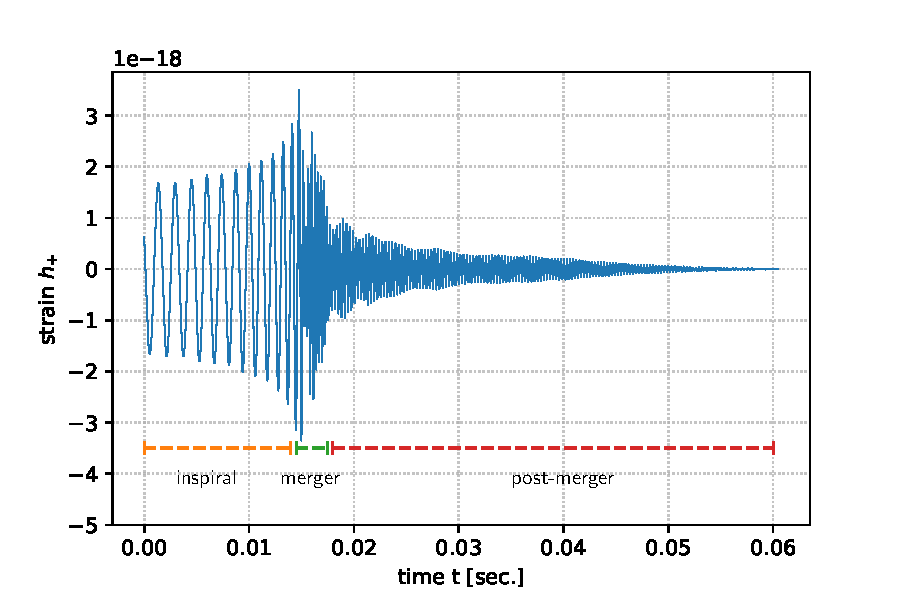
\includegraphics[width=0.45\textwidth]{figures/Capitolo_1/APR4.pdf}
	\end{center}
	\vspace{-11pt}
	\caption{Segnale teorico previsto per per la coalescenza di una BNS con equazione di stato APR4, con una divisione qualitativa tra le diverse fasi}
	\label{fig:forma_onda_APR4}
	\vspace{-20pt}
\end{wrapfigure}
Perciò la fase di spiraleggiamento termina con i due oggetti che si scontrano dando inizio alla fase di coalescenza e quindi, dopo la fusione, alla post-coalescenza, che in base alle proprietà iniziali del sistema può portare a forme d'onda e oggetti diversi.	Mentre la fase di coalescenza dura pochi millisecondi, la fase di post-coalescenza genera un segnale quasi-stazionario. Queste due fasi risultano più complesse da modellare, per cui per il loro studio si fa affidamento a metodi numerici. \cite{maggiore2008gravitational}
%    Cenno sulle equazioni di stato.

I sistemi binari di stelle di neutroni, oltre che ottime sorgenti di onde gravitazionali, risultano anche i migliori scenari per spiegare la fenomenologia dei lampi gamma brevi (short gamma ray burst). I lampi gamma consistono nell'emissione di intensi raggi gamma con uno spettro di durate estremamente vario, per cui si distinguono i short gamma ray burst con durata tipica inferiore a 2s e con un energia media dei fotoni superiore, i long gamma ray burst la quale durata è piccata attorno a 30s, fino agli ultra-long gamma ray burst che arrivano a durare diverse ore, mediamente meno energetici. 
La separazione è legata ai fenomeni fisici che li generano: mentre i GRB lunghi hanno origine nel collasso del nucleo di stelle massive, nel fenomeno della post-luminescenza, la comprensione dell'origine di GRB brevi è risultata più complessa, infatti l'osservazione sperimentale ha portato ad escludere il collasso di stelle massive come origine di tali fenomeni. Candidati plausibili sono risultati invece la coalescenza di BNS o di binarie NS-BH, poiché la durata di GRB brevi richiede strutture compatte con caratteristiche sulla scala dei tempi nell'ordine delle decine di millisecondi, compatibili con la coalescenza di un sistema binario di NS, in particolare l'osservazione di GW170817, evento che si approfondirà nel Capitolo \ref{chapter:gw170817}, mostra come i GRB brevi siano effettivamente legati alla coalescenza di sistemi binari di stelle compatte \cite{maggiore2018gravitational}.
\section{Formazione del corpo celeste}
\label{section:residual}
Ci sono quattro possibili risultati della coalescenza di due stelle di neutroni, in base alle masse delle stelle e dalle loro equazioni di stato. 
Data la massa dell'oggetto $M$, \cite{sarin2020evolution} descrive i possibili stati finali del sistema (Fig.\ref{fig:EvoluzioneBNS}):
\begin{itemize}
	\item $M\gtrsim 1.5 M_{TOV}$\footnote{$M_{TOV}$ è detta massa di Tolman-Oppenheimer-Volkoff e indica la massa massima che può avere una stella di neutroni non rotante}: il sistema collassa immediatamente in un buco nero seguendo il percorso A$\rightarrow$ B$\rightarrow$ C;
\end{itemize}

\begin{itemize}
	\item $1.2 M_{TOV} \lesssim M \lesssim 1.5 M_{TOV}$: l'oggetto rimanente è una stella di neutroni ipermassiva, che collassa in un buco nero in un tempo $\lesssim 1$s, seguendo A$\rightarrow$ B$\rightarrow$ D$\rightarrow$ E;		
	\item $M_{TOV} \lesssim M \lesssim 1.2 M_{TOV}$: rimane una stella di neutroni supermassiva che è destinata a collassare in un buco nero in un tempo di 10 \textdiv $10^4$s, secondo il percorso A$\rightarrow$ B$\rightarrow$ D$\rightarrow$ F$\rightarrow$ G;		\item $M\lesssim M_{TOV}$: rimane una stella di neutroni stabile, secondo il percorso A$\rightarrow$ B$\rightarrow$ D$\rightarrow$ F$\rightarrow$ H.	
\end{itemize}

\vspace{0pt}
\begin{SCfigure}[][ht]
	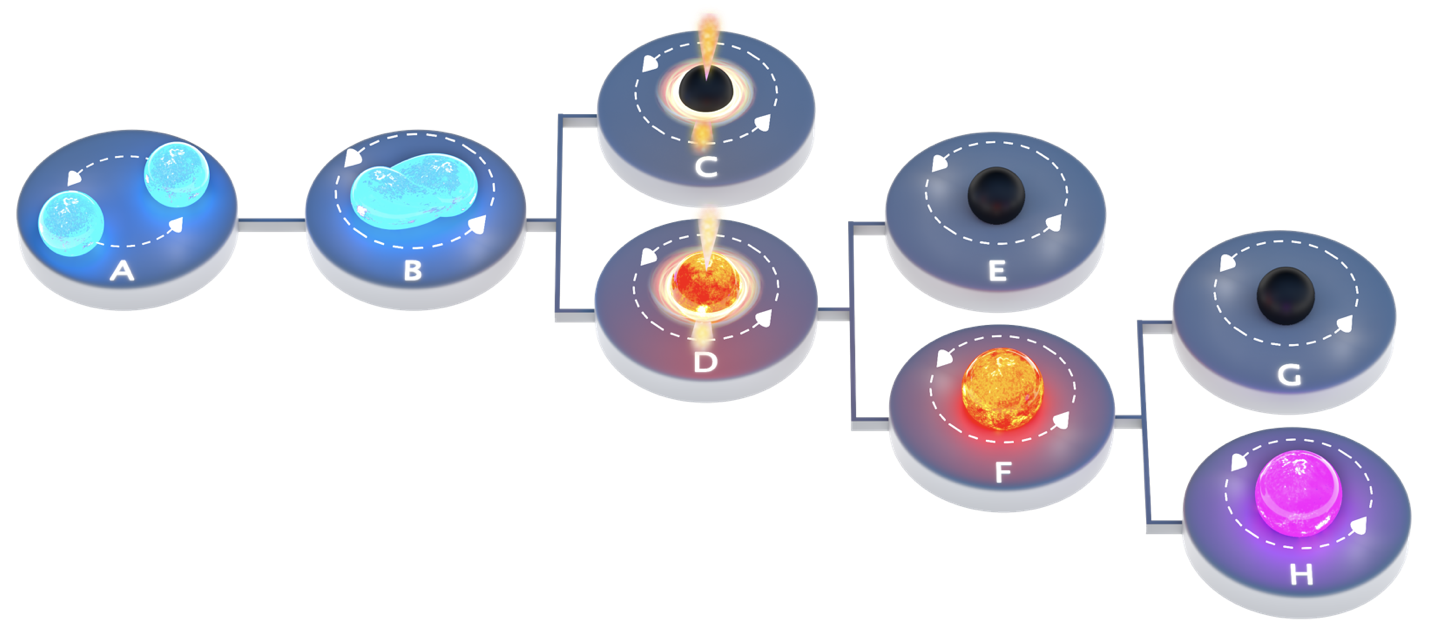
\includegraphics[scale=0.2]{figures/Capitolo_1/MagnetarEvolution.png}
	\captionsetup{width=0.8\textwidth}
	\caption{Rappresentazione pittorica del destino del residuo del merger di un sistema binario di stelle di neutroni, \cite{sarin2020evolution}}
	\label{fig:EvoluzioneBNS}
	\vspace{-20pt}
\end{SCfigure}
%\begin{center}
%	\begin{figure}[ht]
%		\vspace{-20pt}
%		\centering
%		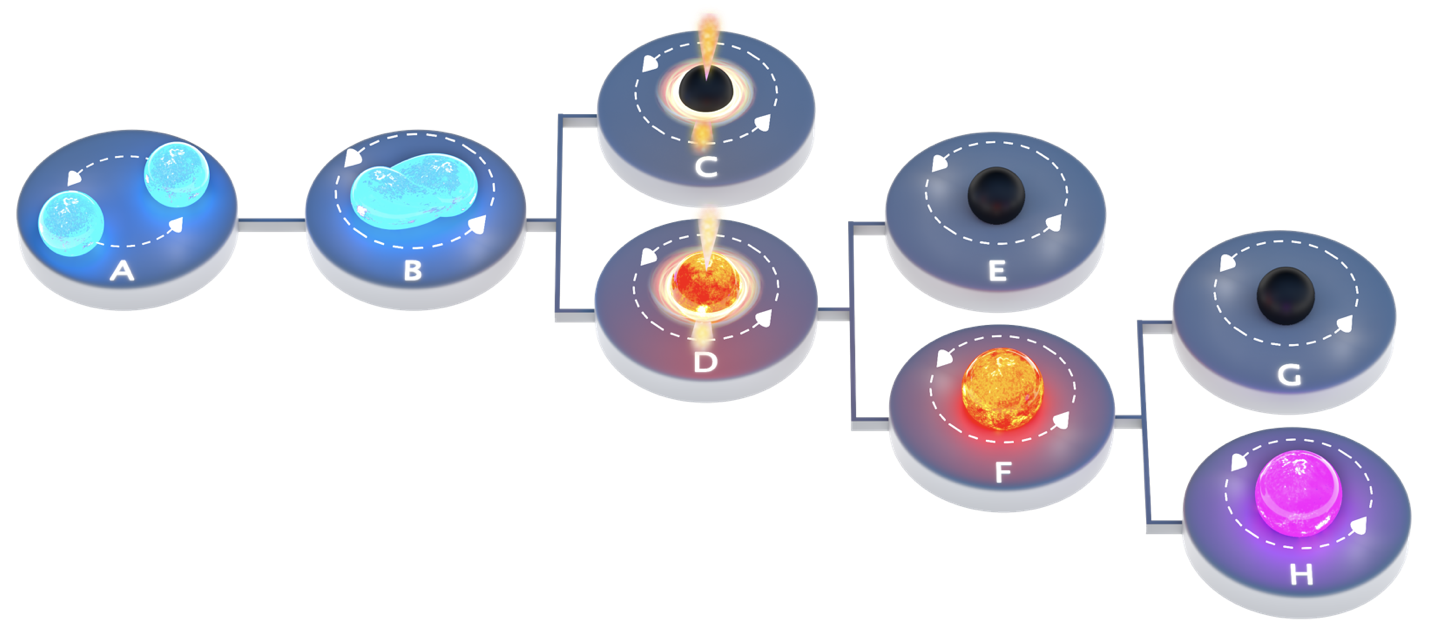
\includegraphics[scale=0.2, angle=0]{figures/Capitolo_1/MagnetarEvolution.png}
%		\setlength{\belowcaptionskip}{-25pt}
%		\caption{Rappresentazione pittorica del destino del residuo del merger di un sistema binario di stelle di neutroni, presa da \cite{sarin2020evolution}}
%		\label{fig:EvoluzioneBNS}
%	\end{figure}
%\end{center}
%Veloce descrizione delle possibili espulsioni di kilonovae

\subsection{Formazione diretta un black hole}	
\label{subsection:Diretto_Black_hole}

%\begin{wrapfigure}{r}{0.45\textwidth}
%	\vspace{-15pt}
%	\begin{center}
%		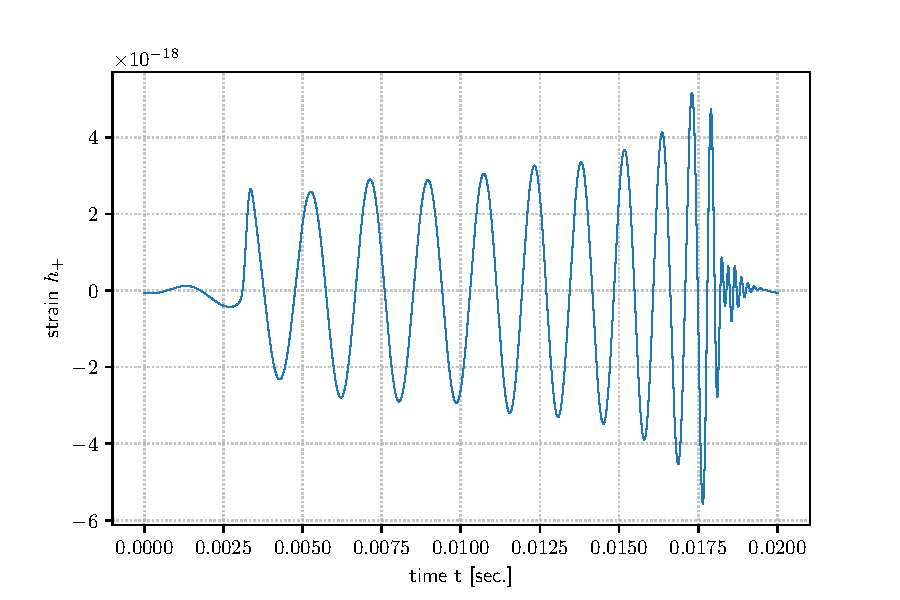
\includegraphics[width=0.5\textwidth]{figures/Capitolo_1/SHT2.2.pdf}
%	\end{center}
%	\vspace{-10pt}
%	\caption{Forma d'onda per la coalescenza di una BNS con equazione di stato SHT2, in cui le masse sono tali da portare il sistema a collassare immediatamente in un BH, producendo nella fase di post merger il ringdown}
%	\label{fig:FormaOndaBH}
%	\vspace{-50pt}
%\end{wrapfigure}
La formazione diretta di un buco nero dopo la coalescenza implica lo spegnimento del segnale, con un collasso quasi sferico che genera delle onde gravitazionali minime\cite{sarin2020evolution}.\\
Questo tipo di segnale ha la particolarità, al contrario degli altri casi di post-merger, di ammattere uno studio analitico attraverso metodi perturbativi relativamente semplici (decrescita esponenziale con un tempo caratteristico legato alla massa del buco nero)\cite{maggiore2018gravitational}.

\subsection{Formazione di una NS ipermassiva}
\label{subsection:ipermassiva}	
La maggior parte delle coalescenze di stelle di neutroni porta alla formazione di stelle di neutroni ipermassive, supermassive o stabili. 

Una stella di neutroni ipermassiva è tale da avere una massa superiore al massimo in massa per una stella rotante uniformemente $M_{TOV}$, ma non collassa per la rotazione differenziale, cioè il fenomeno per cui le sue diverse parti ruotano con velocità angolare differente che permette una maggiore stabilità rispetto a stelle non rotanti o rotanti uniformemente \cite{Baumgarte_2000}, e per il supporto di gradienti termici.
%
%\begin{wrapfigure}{r}{0.45\textwidth}
%	\vspace{-35pt}
%	\begin{center}
%		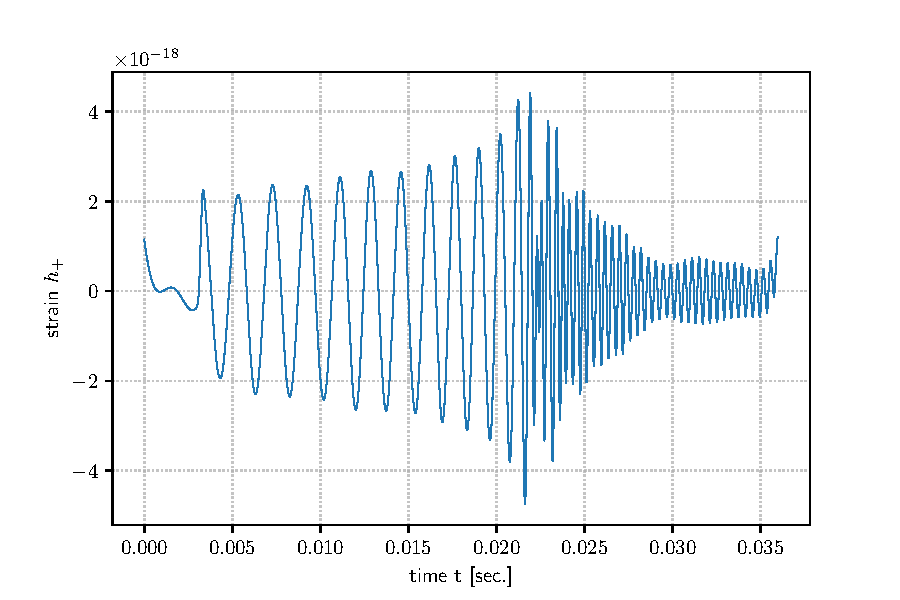
\includegraphics[width=0.5\textwidth]{figures/Capitolo_1/SHT2.0.pdf}
%	\end{center}
%	\vspace{-10pt}
%	\caption{Forma d'onda per la coalescenza di una BNS con equazione di stato SHT2, in cui le masse sono tali da portare il sistema a formare una NS ipermassiva, producendo nella fase di post merger un segnale visibile}
%	\label{fig:FormaOndaToNS}
%	\vspace{-30pt}
%\end{wrapfigure}
Nel momento in cui la stella rallenta la sua rotazione e/o si raffredda e la stella collassa in un buco nero. 
%Nel caso in cui la stella ipermassiva abbia massa tale che $M \gtrsim 1.2 M_{TOV}$ la rotazione uniforme non può dare sufficiente supporto centrifugo per evitare il collasso, per cui la stella collassa non appena la rotazione differenziale termina.
%
%È in generale molto complessa la fisica che regola il collasso dell'ipermassiva residua tuttavia assumendo che per il rilascio del lampo gamma sia necessario tale collasso in buco nero, il ritardo con il quale si è osservato per GW170817, come si vedrà nel capitolo \ref{chapter:gw170817}, può essere, almeno in parte, spiegato con il collasso.
%
%
L'emissione di GW dalla fase di post-coalescenza è attesa avere una quantità di energia rilasciata sotto forma di GW relativamente ampia e confrontabile con il massimo dello spiraleggiamento\cite{sarin2020evolution}. 

\subsection{Formazione di una NS con lunga vita media}
\label{subsection:long_lived}
I residui della post-coalescenza che hanno una massa inferiore a $\smallsim1.2M_{TOV}$ sopravvivono per un tempo superiore al secondo e vengono denomiate supermassive se hanno una massa superiore al limite definito in precedenza $M_{TOV}$, mentre per valori inferiori sono stabili.
È importante osservare in Figura \ref{fig:EvoluzioneBNS} che per entrambi i prodotti finali si passa comunque per una fase di forte rotazione differenziale immediatamente successiva alla coalescenza rendendo i metodi di ricerca di segnali di GW non differenti da quelli per il caso di residuo ipermassivo.
L'osservazione sperimentale mostra che questo tipo di esito si presenta in un numero non trascurabile di casi.

Come detto, le simulazioni mostrano che stelle supermassive generate dalla coalescenza di un sistema binario di stelle di neutroni hanno una vita compresa tra $\smallsim10$s e $\smallsim10^4$s. In realtà l'osservazione sperimentale mostra che queste stelle tendono a collassare in una scala di tempi più breve di quella attesa e tale discrepanza si pensa possa includere eccessi di energia emessa in onde gravitazionali nelle prime fasi, o quark liberi che portano a modifiche nel momento di inerzia della stella rispetto al caso con materia ordinaria\cite{sarin2020evolution}.\\
Questi vincoli hanno grande importanza, soprattutto per la ricerca futura: il fatto che le stelle di neutroni nascenti siano composte da quark non confinati suggerisce che vi sia una transizione di fase adrone-quark dipendente dalla temperatura e, comprendere dove avvenga questa transizione nel diagramma di fase nucleare è un informazione chiave per dedurre informazioni sul comportamento della materia nucleare e di conseguenza sull'equazione di stato.
Il fatto, invece, che le NS supermassive rallentino la rotazione soprattutto a causa dell'emissione di GW ha importanti conseguenze per la dinamica della NS stessa e permette di avere vincoli sull'energia per ricostruire la natura dell'oggetto residuo nelle future analisi\cite{sarin2020evolution}.
%neutrino emissions, thermal evolution, dynamical evolution, elettromagnetic observations?

%DA CANCELLARE(?)[Per le NS a lunga vita si conoscono le emissioni elettromagnetiche, mentre per le emissioni di onde gravitazionali la conoscenza del fenomeno risulta ancora incompleta: non si conosce con certezza la gerarchia di importanza dei meccanismi, per quanto tempo rimangono attive o quanta energia viene emessa. Le tre principali instabilita rilevanti per la produzione di GW sono le instabilità di spin-flip, di bar-mode e r-mode.
%L'instabilità precessionale spin-flip, legata al cambiamento di rotazione di un oggetto rotante, porta la nascente NS ad essere un "rotatore ortogonale" e quindi un ottimo emettitore di GW.
%L'instabilità bar-mode si presenta in due varietà: dinamica, che è attiva nel primo secondo della vita della NS, e secolare, che ha maggiore importanza nel lungo periodo. 
%Infine gli r-mode, ovvero oscillazioni toroidali a bassa frequenza per le quali la forza di Coriolis è la "forza di ripristino"\cite{sarin2020evo5lution}.]
\section[Frequenze caratteristiche]{Frequenze  di coalescenza e post-coalescenza di un'ipermassiva}
\label{section:frequenze_caratteristiche}
\begin{wrapfigure}{r}{0.45\textwidth}
	\vspace{-25pt}
	\begin{center}
		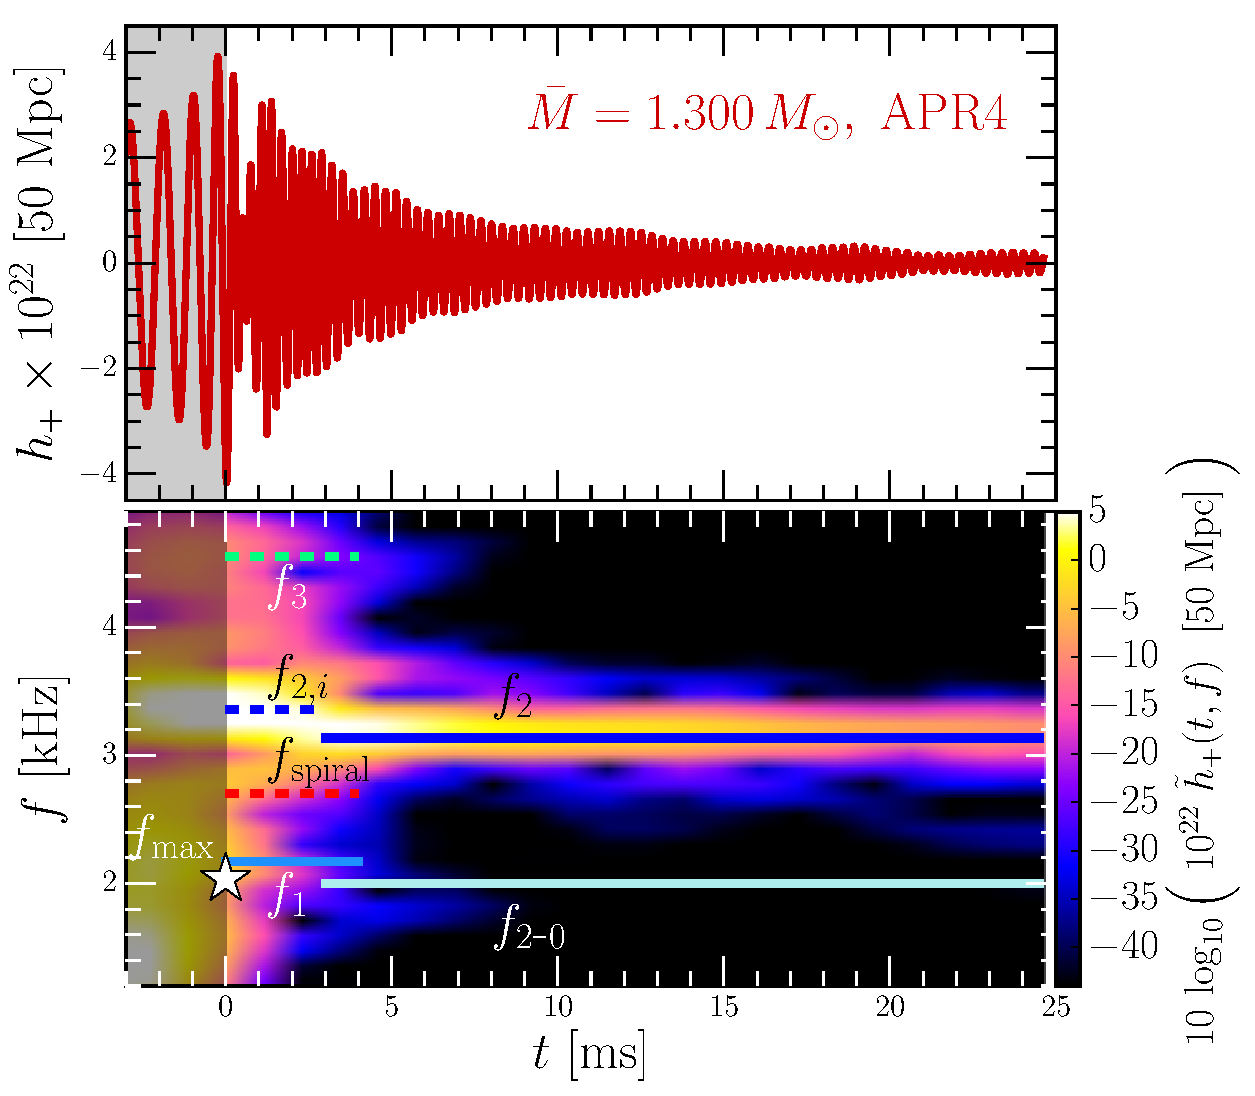
\includegraphics[width=0.45\textwidth]{figures/Capitolo_1/GW_spectrogram_APR4-q10-M1300.pdf}
	\end{center}
	\vspace{-10pt}
	\caption{Forma d'onda e relativo spettrogramma per la post-coalescenza di una BNS con equazione di stato APR4 (morbida), \cite{Rezzolla_2016}}
	\label{fig:spettrogramma_postmerger_APR4}
	\vspace{-20pt}
\end{wrapfigure}
%\begin{wrapfigure}{r}{0.45\textwidth}
%	\vspace{-15pt}
%	\begin{center}
%		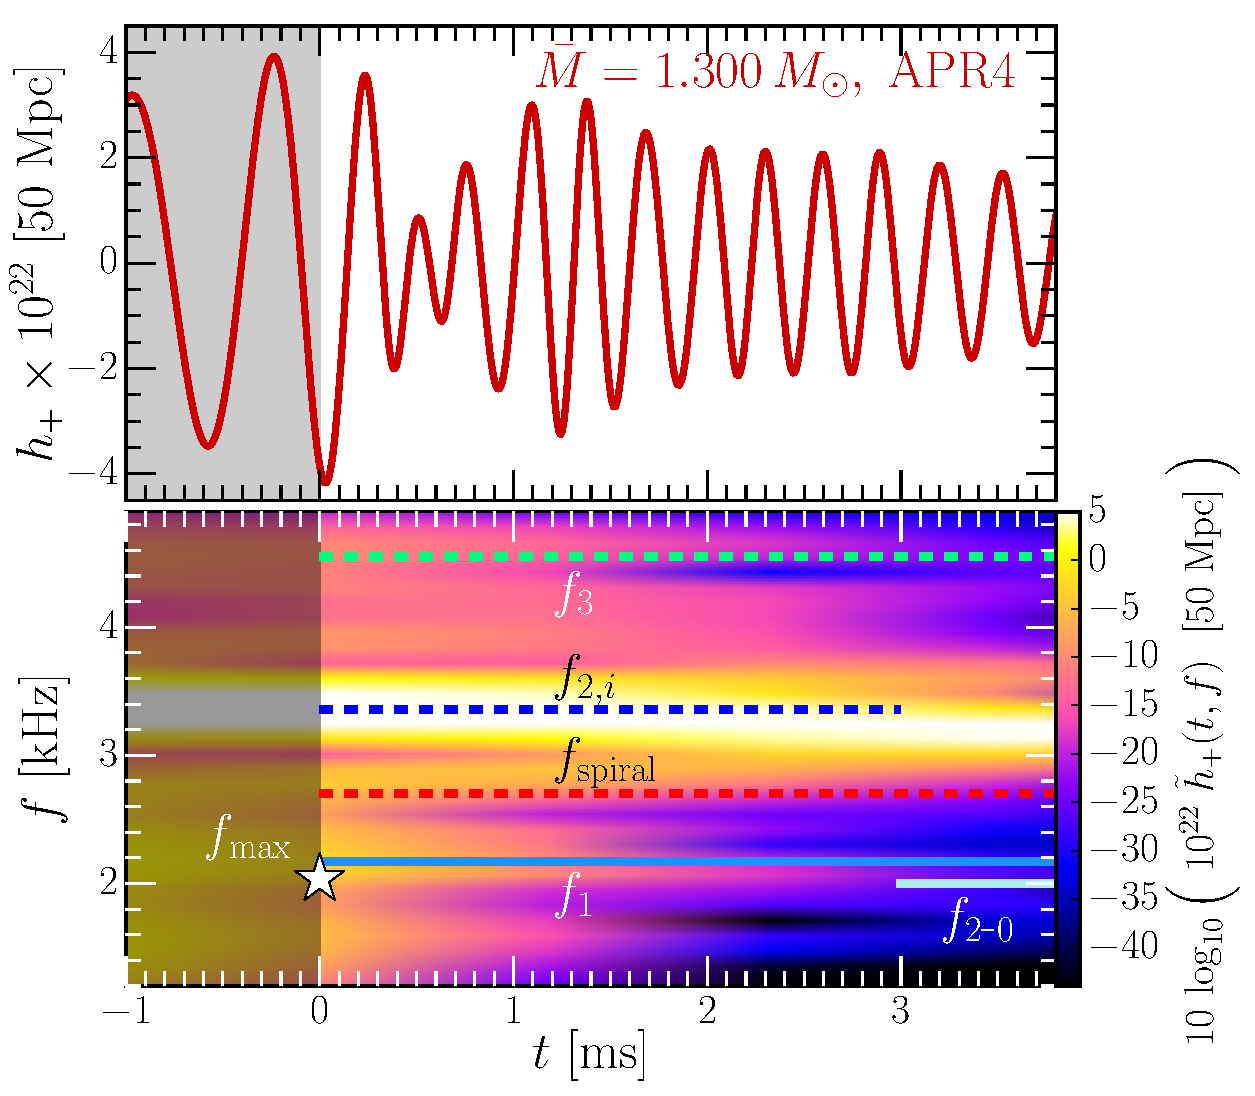
\includegraphics[width=0.5\textwidth]{figures/Capitolo_1/GW_spectrogram_short_APR4-q10-M1300.pdf}
%	\end{center}
%	\vspace{-10pt}
%	\caption{Forma d'onda e relativo spettrogramma per la coalescenza di una BNS con equazione di stato APR4 (morbida), \cite{Rezzolla_2016}}
%	\label{fig:spettrogramma_merger_APR4}
%	\vspace{-20pt}
%\end{wrapfigure}
%Una BNS realistica presenta una massa compresa tra $\smallsim\SI{2.4}{\solarmass}$ e $\smallsim\SI{2.8}{\solarmass}$ e una differenza tra le due componenti che è di $\smallsim20\%$ o minore.
A partire dal segnale di GW, in particolare nelle fasi di coalescenza e post-coalescenza, possono essere ottenute informazioni sull'equazione di stato della materia a densità nucleare e, da un'analisi spettrale, informazioni sulla deformabilità mareale delle due stelle.\\
Simulazioni numeriche relativistiche di coalescenza di BNS e l'evoluzione della post-coalescenza mostra che l'emissione di GW da un residuo ipermassivo è legato alla EOS e può trovarsi a frequenze comprese tra $\smallsim2$ e 4kHz, ed è fortemente correlato con la compattezza e la deformabilità mareale delle stelle. Questa correlazione, con quantità calcolate per stelle di neutroni fredde e non rotanti, stato in cui non si trova l'ipermassiva residua, suggerisce come gli effetti dovuti a rotazione e temperatura giochino un ruolo limitato nelle proprietà del segnale di onda gravitazionale e mostra come la misura del modo dominante nella frequenza del post-merger possa portare a una importante misura dell'equazione di stato nucleare\cite{sarin2020evolution}.\\
Considerando dunque il segnale gravitazionale dovuto alla coalescenza di due stelle di neutroni, con una differneza di massa inferiore al 20\%, si possono riassumere le proprietà fondamentali come descritto in \cite{Rezzolla_2016}:
\begin{itemize}
	\item la frequenza della GW al massimo di ampiezza $f_{max}$ è legata in modo quasi-universale con la deformabilità mareale delle due stelle;
	\item le frequenze $f_1$, $f_{2,i}$ e $f_3$ rappresentano i picchi principali visibili dall'osservazione della post-coalescenza, tra le quali si ottiene la seguente relazione empirica: $f_{2,i}\simeq\frac{f_1 + f_3}{2}$. Il picco $f_1$ è legato alla compattezza delle stelle, mentre il picco $f_{2,i}$ è legato al raggio della configurazione non rotante più massiva e corrisponde al modo fondamentale della NS ipermassiva con $l=2=m$;
	\item si identifica in alcuni casi un altro picco $f_{2-0}$ che si riferisce all'accoppiamento tra il modo fondamentale con $l=2=m$ e il modo con simmetria assiale, cioè con $l=2$ e $m=0$;
	\item il picco $f_{spiral}$ associato alla deformazione spiraleggiante dovuta alla rotazione, è però impossibile da misurare in calcoli numerici e si utilizzano dunque i valori prodotti da considerazioni analitiche. Si nota infine che $f_{spiral}$ coincide per molte EOS (in particolare EOS rigide) con la frequenza $f_1$, mentre per altre (EOS morbide) non si ha questa corrispondenza.
\end{itemize}

Nella fase di post-coalescenza, nei casi in cui il sistema non collassa immediatamente in un buco nero, evidenziando nella forma d'onda una fase di ringdown in cui il segnale si spegne, l'unica frequenza a sopravvivere è il picco $f_2$, spariscono gli altri picchi, lasciando solo $f_{2-0}$ a basse energie, come si osserva in Figura \ref{fig:spettrogramma_postmerger_APR4}.

È poi possibile trovare diverse relazioni quantitative che legano le frequenze osservate con le proprietà stellari, che risultano particolarmente utili come verifica delle previsioni teoriche.

%	% !TEX root = ../../Tesi_Triennale_PMNS.tex
\chapter[Osservazione di GW da BNS]{GW170817: osservazione di onde gravitazionali prodotte da un sistema binario di stelle di neutroni}
\label{chapter:gw170817}
Rivelato il 17 Agosto 2017 dal network LIGO-Virgo, GW170817 è il primo segnale di onda gravitazionale generato dallo spiraleggiamento un sistema binario di stelle di neutroni.
Il segnale osservato, alla fine del secondo run di misure O2, è tutt'ora il più energetico osservato tra questi tipi di segnale, con un rapporto segnale su rumore (SNR) di 32.4.

Oltre al segnale di GW è stato osservato un gamma ray burst, dopo 1.7s dalla coalescenza.
\section{Osservazione dello spiraleggiamento}
\label{section:osservazioneInspiralGW170817}
\begin{wrapfigure}{r}{0.5\textwidth}
	\vspace{-15pt}
	\begin{center}
		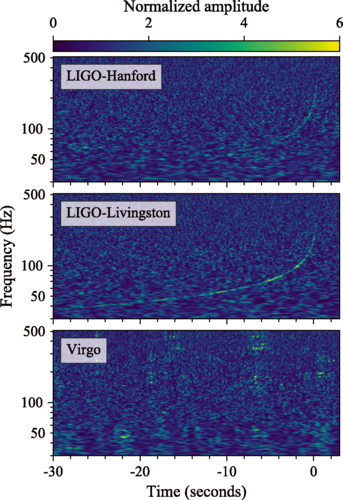
\includegraphics[width=0.4\textwidth]{figures/Capitolo_2/gw170817_time_freq.png}
	\end{center}
	\vspace{-5pt}
	\caption{Segnali in una mappa tempo frequenza nel network di detectors, presa da \cite{Abbott_2017a}}
	\label{fig:osservazione_gw170817}
	\vspace{-40pt}
\end{wrapfigure}
Dalla rappresentazione tempo-frequenza dei dati, a cui viene sottratto il rumore e sbiancati, si può notare immediatamente che il segnale che, idealmente deve presentare la forma di un chirp, è ben visibile nei due rivelatori LIGO, meglio in Livingston che in Hanford, mentre in Virgo, a causa della posizione celeste della sorgente del segnale, non è possibile distiguere visivamente nessun pattern rispetto rumore di fondo. La (non) rivelazione risulta comunque utile, soprattutto per permettere l'individuazione della posizione celeste della sorgente.

L'analisi del'evento mostra un segnale coerente nei due detector LIGO, grazie al quale si individua la sorgente in una regione identificata da un angolo solido di 31 $\text{deg}^2$, che a sua volta ha permesso l'identificazione della controparte elettromagnetica GRB170817A. 
Si è ottenuto inoltre un SNR combinato tra i detector di 32.4 che rendono questo segnale il più intenso rivelato finora.\cite{Abbott_2017a}

\subsection{Proprietà della sorgente}
\label{subsection:proprietàSorgGW170817}
La relatività generale fa previsioni abbastanza dettagliate sull'evoluzione della frequenza, che è legata, nella prima fase, a una combinazione delle masse delle stelle progenitrici, detta massa di chirp 
\begin{equation}
	\mathcal{M} = \frac{(m_1m_2)^{3/5}}{(m_1+m_2)^{1/5}}
	\label{eqn:chirpmass}
\end{equation}
Nelle fasi più avanzate, le orbite si stringono e aumenta la frequenza dell'onda gravitazionale, mentre la fase della GW è sempre più influenzata da effetti relativistici legati al rapporto tra le masse $q = m_2/m_1$ e dagli accoppiamenti spin-orbita e spin-spin. 
La composizione interna degli oggetti diventa importante quando la distanza tra essi diventa paragonabile alle dimensioni dell'oggetto stesso. 

Le proprietà della sorgente di onde gravitazionali sono ottenute dal confronto con le forme d'onda predette dalla teoria. Viene fatta dunque una analisi Bayesiana nel range di frequenze 30-2048Hz che include gli effetti dell'incertezza di calibrazione di $1\sigma$ sul segnale ricevuto.
\begin{wrapfigure}{r}{0.5\textwidth}
	\vspace{-0pt}
	\begin{center}
		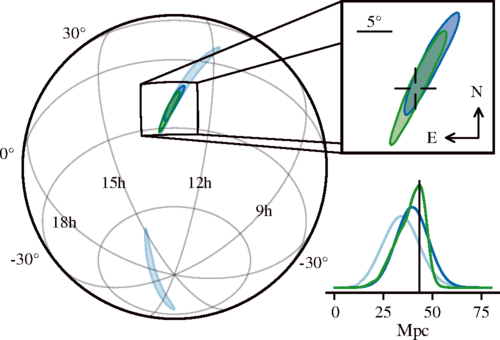
\includegraphics[width=0.5\textwidth]{figures/Capitolo_2/skymap.png}
	\end{center}
	\vspace{-5pt}
	\caption{Sky location ricostruita per GW170817, nella versione preliminare in blu chiaro per Hanford-Livingston e in blu scuro per Handord-Livingston-Virgo, mentre nella versione finale in verde, presa da \cite{Abbott_2019}}
	\label{fig:skymap}
	\vspace{-10pt}
\end{wrapfigure}
La sorgente viene in questo modo identificata in una regione celeste di 28$\text{deg}^2$ di area e $380\text{Mpc}^3$ di volume, utilizzando una combinazione di timing, fase e ampiezza dei tre detector. La distanza luminosa, la più prossima osservata finora, viene individuata in $40_{-14}^{+8}$Mpc. Per le masse delle stelle compatte risulta più semplice dedurre la massa di chirp, indipendente dalla scelta della prior nell'analisi Bayesiana legata all'equazione di stato scelta per le stelle progenitrici, che si valuta in $\mathcal{M}=1.188_{-0.002}^{+0.004}$, rispetto alle masse singole, che soffrono invece della degenerazione tra il rapporto tra le masse $q$ e le componenti dello spin $\chi_1$ e $\chi_2$. È necessario fare quindi assunzioni a partire dalle EOS che si considerano, ottenendo dei range $m_1 \in (1.36, 2.26)M_\odot$ e $m_2 \in (0.86, 1.36)M_\odot$ evidentemente meno precisi, ma comunque utili come evidenza della natura di stelle di neutroni del sistema binario, escludendo invece la possibilità di buchi neri che prevederebbe range di masse superiori\cite{Abbott_2017a}.

%QUALCOSA SULLE TIDAL DEFORMABILITIES?
\section{Ricerca del post-merger del residuo}
\label{section:postmergerGW170817}
L'analisi del post-merger, atteso in seguito all'osservazione del segnale GW170817, non ha portato ad evidenza statisticamente significativa di un oggetto in seguito alla coalescenza, ma ha permesso di ottenere informazioni sul limite superiore sulle ampiezze di strain ed energie di GW osservabili. Gli attuali detector infatti non sono calibrati in modo tale da permettere rivelazioni alle alte frequenze del post-merger.

Mentre lo studio del segnale elettromagnetico associato alla GW non permette di escludere nessuno dei possibili stati finali indicati in sezione \ref{section:residual}, grazie ai valori ottenuti per le masse dei progenitori date nella sezione \ref{subsection:proprietàSorgGW170817} si calcola che per un ampio range di equazioni di stato la coalescenza produce uno stato di NS ipermassiva. Questo spiega anche il ritardo del lampo gamma rispetto all'istante di rivelazione del segnale di merger. 

Come si vedrà nella sezione \ref{section:analisiSimSingole} in base alla EOS che si considera si ottiene un contributo diverso nel post-merger che inizia attorno a $\smallsim1$kHz. Più in generale, oltre alla EOS hanno fondamentale importanza le masse e gli spin degli oggetti iniziali. 
Per quanto riguarda invece la rivelazione di questa fase del segnale, anche considerando modelli ottimistici da stati finali di NS ipermassiva o supermassiva, l'SNR atteso per distanze di $\smallsim40$Mpc è $\smallsim1-2$ ordini di grandezza più piccolo di quello rivelabile dal network LIGO-Virgo attualmente utilizzato, facendo uso di algoritmi di confronto con segnali modellati (che comunque sono meno utilizzati per il post-merger, per la difficoltà nel modellare questa fase del segnale).
Si ipotizza tuttavia che nei prossimi run la sensibilità del network sarà tale da permettere la rivelazione di queste emissioni\cite{Abbott_2017b}.

Come si può osservare in figura \ref{fig:NoiseFrequenze} i tre detector del network hanno zone diverse di sensibilità, in particolare si nota che in generale la sensibilità diminuisce significativamente ad alte frequenze. Il rumore di LIGO Hanford è più alto rispetto a Livingston nella banda di frequenza compresa tra 100Hz e 1kHz, mentre Virgo ha sofferto grandi fluttuazioni di rumore e proprietà spettrali non stazionarie a frequenze superiori a 2.5kHz.
\begin{wrapfigure}{r}{0.5\textwidth}
	\vspace{-0pt}
	\begin{center}
		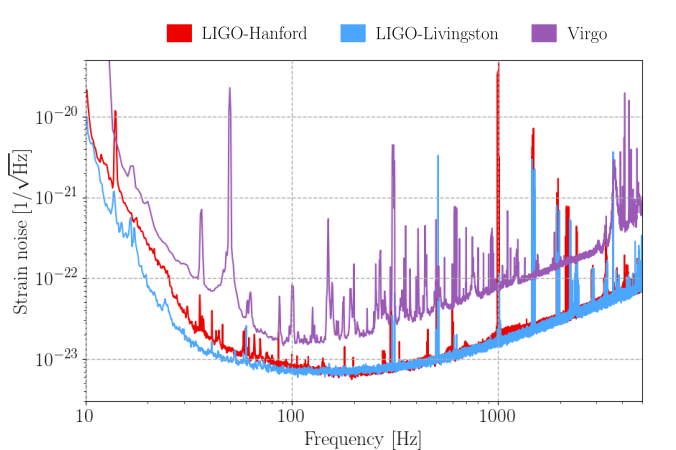
\includegraphics[width=0.5\textwidth]{figures/Capitolo_2/noiseData.png}
	\end{center}
	\vspace{-5pt}
	\caption{Sensibilità di ciascun rivelatore durante il run O2, indicata dall'ampiezza del rumore di strain in funzione della frequenza, presa da \cite{Abbott_2019}}
	\label{fig:NoiseFrequenze}
	\vspace{-10pt}
\end{wrapfigure}
Per l'analisi sono stati usati due diversi algoritmi, in base al tipo di segnale ricercato: per segnali di brave durata è stato usato cWB (Coherent Wave Burst) utilizzando i dati di LIGO tra 1024Hz e 4096Hz, mentre per i segnali di durata intermedia si è utilizzato l'algoritmo STAMP (Stochastic Transient Analysis Multidetector Pipeline) nelle frequenze comprese tra 24Hz e 2000Hz e tra 2000Hz e 4000Hz nei dati di LIGO, mentre cWB con i dati del network LIGO-Virgo ricerca le frequenze tra 24Hz e 2048Hz. 

Per la ricerca di segnali con incertezze teoriche cosi grandi risulta inefficiente l'utilizzo di metodi di ricerca matched-filtering, ovvero metodi che utilizzano segnali di forme conosciute e, attraverso funzioni di filtraggio escludono la componente di rumore; in particolare si sceglie la funzione che massimizza il rapporto segnale su rumore (SNR) per tale segnale\cite{maggiore2008gravitational}. È immediato comprendere che non conoscendo con certezza la forma che deve assumere il segnale questo metodo risulta inefficace per la ricerca del post-merger. Gli algoritmi che si usano invece ricercano eccessi di potenza in una mappa tempo-frequenza e, usando metodi di riconoscimento dei pattern, possono identificare la presenza di segnali di GW nelle mappe. In particolare gli algoritmi sono tali da considerare i dati del network e non dei singoli rivelatori, utilizzando tecniche che permettono di combinare coerentemente i dati dei singoli detector e dare risposte differenti a forme d'onda diverse.

Come anticipato, la ricerca viene divisa tra segnali brevi ($\lesssim$1s) e intermedi ($\lesssim$500s).
\subsection{Segnali brevi}
L'analisi dei segnali brevi, ad alte frequenze viene fatta con l'algoritmo cWB e consiste nella ricerca di eccessi di potenza nell'intervallo di 2s che precede il segnale elettromagnetico GRB 170817a, in un intervallo che comprende quindi anche il merger.
In particolare l'algoritmo valuta la massima verosimiglianza di eccessi di potenza in una trasformata di wavelet a multi-risoluzione per ogni detector, classificando gli eventi in una gerarchia di SNR. La significanza degli eventi è data dal confronto con la distribuzione del fondo stocastico, che è generata con metodi che saranno precisati nel capitolo \ref{chapter:cwb}. 

È convenzione esprimere la sensibilità della ricerca di una data forma d'onda in $h_{rss}^{50\%}$, ovvero la somma in quadratura delle ampiezze di strain di segnali che sono rivelati con un'efficienza del 50\%. La quantità $h_{rss}$ è definito come
\begin{equation}
	h_{rss} = \sqrt{2\int_{f_{min}}^{f_{max}}df(|\tilde{h}_+(f)|^2 + |\tilde{h}_\times(f)|^2 )}
\end{equation}
dove $f_{min}$ e $f_{max}$ sono rispettivamente le frequenze massima e minima sulle quali si effettua la ricerca. 
Il criterio su $h_{rss}^{50\%}$ scelto per questo metodo di ricerca è tale da avere una probabilità di falso allarme di $10^{-4}$.

Per evitare la possibile perdita di segnali di EOS rigide, si fa la scelta conservativa di ricercare segnali a partire da 1024Hz, nonostante tutte le forme d'onda abbiano emissioni dominanti molto al di sopra di tale soglia.

In conclusione, non viene trovata evidenza di nessun segnale di GW in questa banda di frequenze.
L'ampiezza di strain per produrre una probabilità del 50\% di rivelazione di un segnale è compresa tra $2.1 \times 10^{-22} \text{Hz}^{-1/2}$ e $3.5 \times 10^{-22} \text{Hz}^{-1/2}$. L'energia irradiata da un sorgente che emette isotropicamente è data da 
\begin{equation}
	E_{gw}^{iso} = \frac{\pi c^3}{2G}\mathcal{D}^2\int d\Omega \int_{f_{min}}^{f_{max}}dff^2(|\tilde{h}_+(f)|^2 + |\tilde{h}_\times(f)|^2 ) \approx \frac{\pi^2 c^3}{G}\mathcal{D}^2\bar{f}^2h_{rss}^2
\end{equation}
con $\mathcal{D}$ è la distanza dalla sorgente e $\bar{f}$ è la frequenza caratteristica data da 
\begin{equation}
	\bar{f} = \frac{2}{h_{rss}^2}\int_{f_{min}}^{f_{max}}dff(|\tilde{h}_+(f)|^2 + |\tilde{h}_\times(f)|^2 )
\end{equation}

In questo modo si ottiene un range di energie rivelabili secondo il criterio del $h_{rss}^{500\%}$ è dato da $4.8-\SI{19.6}{\solarmass}c^2$, al di fuori delle masse in gioco per BNS, per cui non è possibile con i rivelatori attuali rivelare le emissioni di GW di NS ipermassive associate a GW170817.
\subsection{Segnali di durata intermedia}
Per segnali di durata intermedia si utilizzano i due algoritmi cWB e STAMP, concentrando la ricerca in una zona limitata dello spazio, indicata dalla controparte elettromagnetica che permette di evitare trigger accidentali.

Sono considerate due morfologie di forme d'onda corrispondenti a GW da bar-modes secolari o causati da elicità causate dal campo magnetico nella stella nascente. I meccanismi di emissione attraverso modi-r non sono considerati per la durata che richiederebbe scale temporali più lunghe.
Approfondire?

Nell'analisi di STAMP, che ricerca segnali in uno spettrogramma con pixel di 1s$\times$1Hz, creati con la correlazione incrociata dei dati di detector spazialmente separati, sia con metodi seed-based clustering, dove per seed si intendono pixel con un eccesso di potenza sopra una certa soglia che vengono connessi formando un cluster, sia con algoritmi seedless, senza quindi applicare soglie minime, per il riconoscimento dei pattern, non viene trovato nessun significativo eccesso di potenza, con una probabilità di falso allarme di $10^{-2}$.

L'analisi con cWB è invece analoga alla precedente, ma considera un intervallo di tempo che parte dal merger e copre 1000s. Anche in questo caso, con probabilità di falso allarme di $10^{-4}$ nessun candidato è trovato nella banda di frequenza considerata.

Concludendo, non viene trovata nessuna evidenza di un segnale di post merger nei dati considerati: se esiste un segnale questo è comunque troppo debole per essere rivelato dai rivelatori nel run O2 \cite{Abbott_2017b}.

\section{Sugli altri eventi rivelati}
\subsection*{GW190425}
Il secondo evento rivelato di inspiral di BNS è GW190425 durante il run O3 del network Virgo-LIGO. In realtà durante l'evento il detector LIGO Hanford era spento, quindi il network contava solo su due rivelatori e la soglia di SNR per Virgo era inferiore alla soglia minima. Non sono inoltre stati rivelati segnali elettromagnetici associati all'evento.

L'evento ha avuto un SNR di 12.9 per LIGO Livingston mentre di solo 2.5, ovvero sotto la soglia di trigger pari a 4, per Virgo. La differenza tra i due rivelatori è consistente con la differenza di sensibilità tra i due detector\cite{Abbott_2020b}.

\paragraph{Proprietà della sorgente} In continuità con le definizioni fatte per le proprietà del segnale GW170817, si riportano brevemente le caratteristiche del segnale GW190425.

Si individua la sorgente in un'area celeste di 8284deg$^2$ al 90\% di credibilità (estremamente più impreciso di GW170817) e la distanza viene valutata in $159_{-71}^{+69}$Mpc. La così più grande incertezza rispetto al primo segnale è dovuta al minor numero di detector coinvolti e all'impossibilità di escludere regioni grazie alla controparte elettromagnetica che non viene rivelata in questo caso.
La massa di chirp è pari a $1.4873^{+0.0008}_{-0.0006}M_\odot$, mentre le masse delle stelle progenitrici sono $m_1 \in (1.60, 2.52)M_\odot$ e $m_2 \in (1.46, 1.68)M_\odot$\cite{Abbott_2020b}.

%\begin{wrapfigure}{r}{0.5\textwidth}
%	\vspace{-5pt}
%	\begin{center}
%		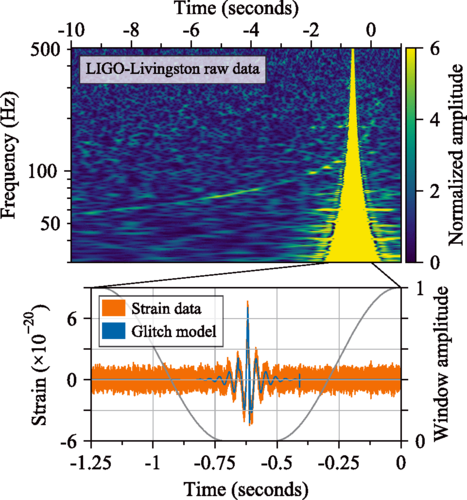
\includegraphics[width=0.5\textwidth]{figures/Capitolo_2/signal.png}
%	\end{center}
%	\vspace{-5pt}
%	\caption{\cite{Abbott_2017b}}
%	\label{fig:signalInspiral}
%	\vspace{-10pt}
%\end{wrapfigure}
%	% !TEX root = ../Tesi_Triennale_PMNS.tex
\chapter[cWB]{cWB: proprietà dell'algoritmo per la rivelazione e la ricostruzione di segnali di onde gravitazionali}
\label{chapter:cwb}
\begin{center}
	$\smallsim 5/6$ pagine
\end{center}

Introduzione sull'algoritmo fatta nel paragrafo precedente, magari riprenderla velocemente.

Coherent analysis, significato e descrizione della likelihood: spiega quindi bene la differenza con gli algoritmi classici di confronto con segnali già modellati.

regolatori, antenna pattern

algoritmi utilizzati: wavelet transformation, (linear predicion error), mappa verosimiglianza, mappa energia coerente (con piccoli grafici esemplificativi)

(cenni sulla trasformazione di fase)


\lipsum[3]\cite{Abbott_2017a}.

\lipsum[4]\cite{Klimenko_2008}.

\lipsum[6]\cite{Klimenko_2016}.

%	% !TEX root = ../../Tesi_Triennale_PMNS.tex
\chapter{Analisi}
\label{chapter:analisi}
\section{Primo approccio all'algoritmo}
\label{section:analisiSimSingole}
\begin{center}
	$\smallsim 2/3$ pagine
\end{center}

\lipsum[7]\cite{hartle2003gravity}.

\begin{center}
	\begin{figure}[H]
		\centering
		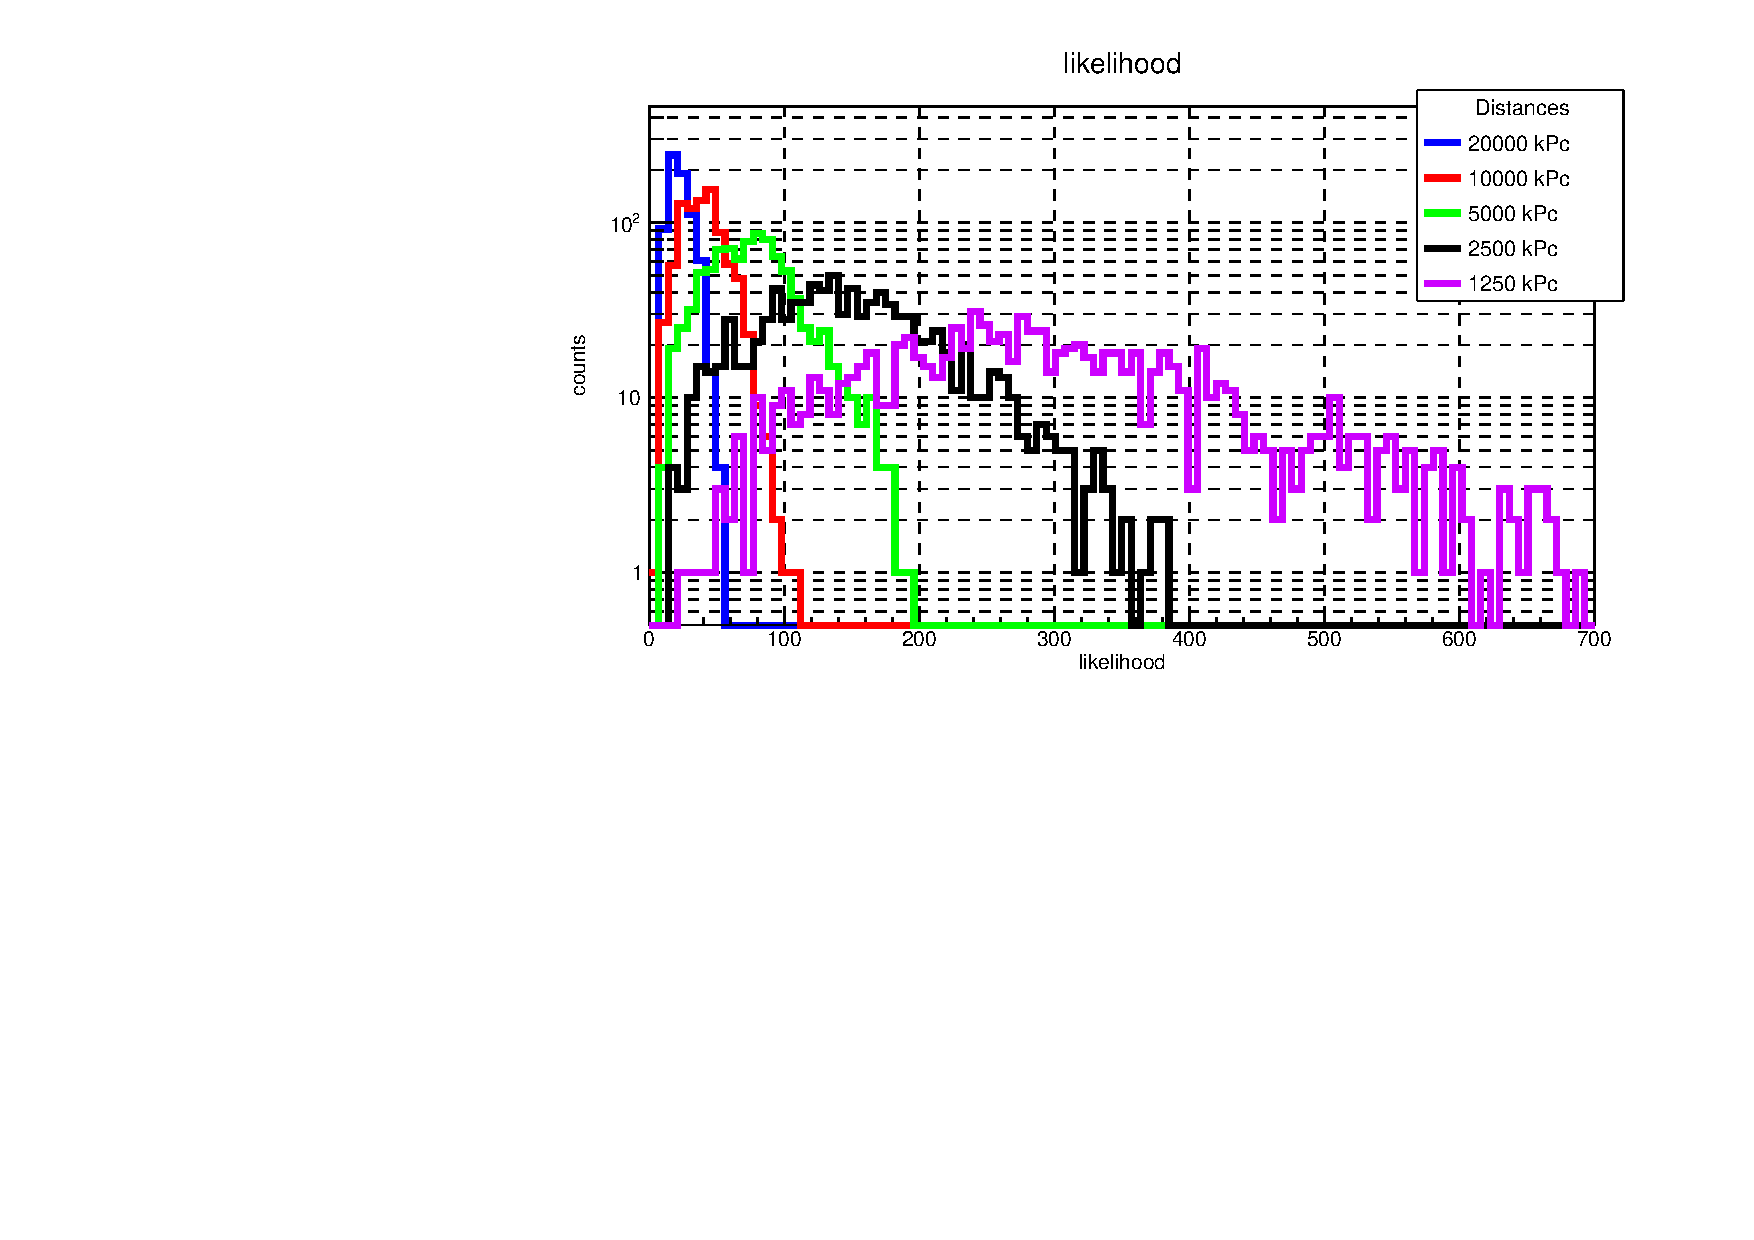
\includegraphics[scale=0.8, angle=0]{figures/Capitolo_4/likelihoodDistribution.pdf}
		\setlength{\belowcaptionskip}{-20pt}
		\caption{}
		\label{fig:likelihoodDistribution}
	\end{figure}
\end{center}	

\section{Ricerca frequenza post-merger}
\begin{center}
	$\smallsim 5/6$ pagine
\end{center}

\begin{center}
	\begin{figure}[H]
		\centering
		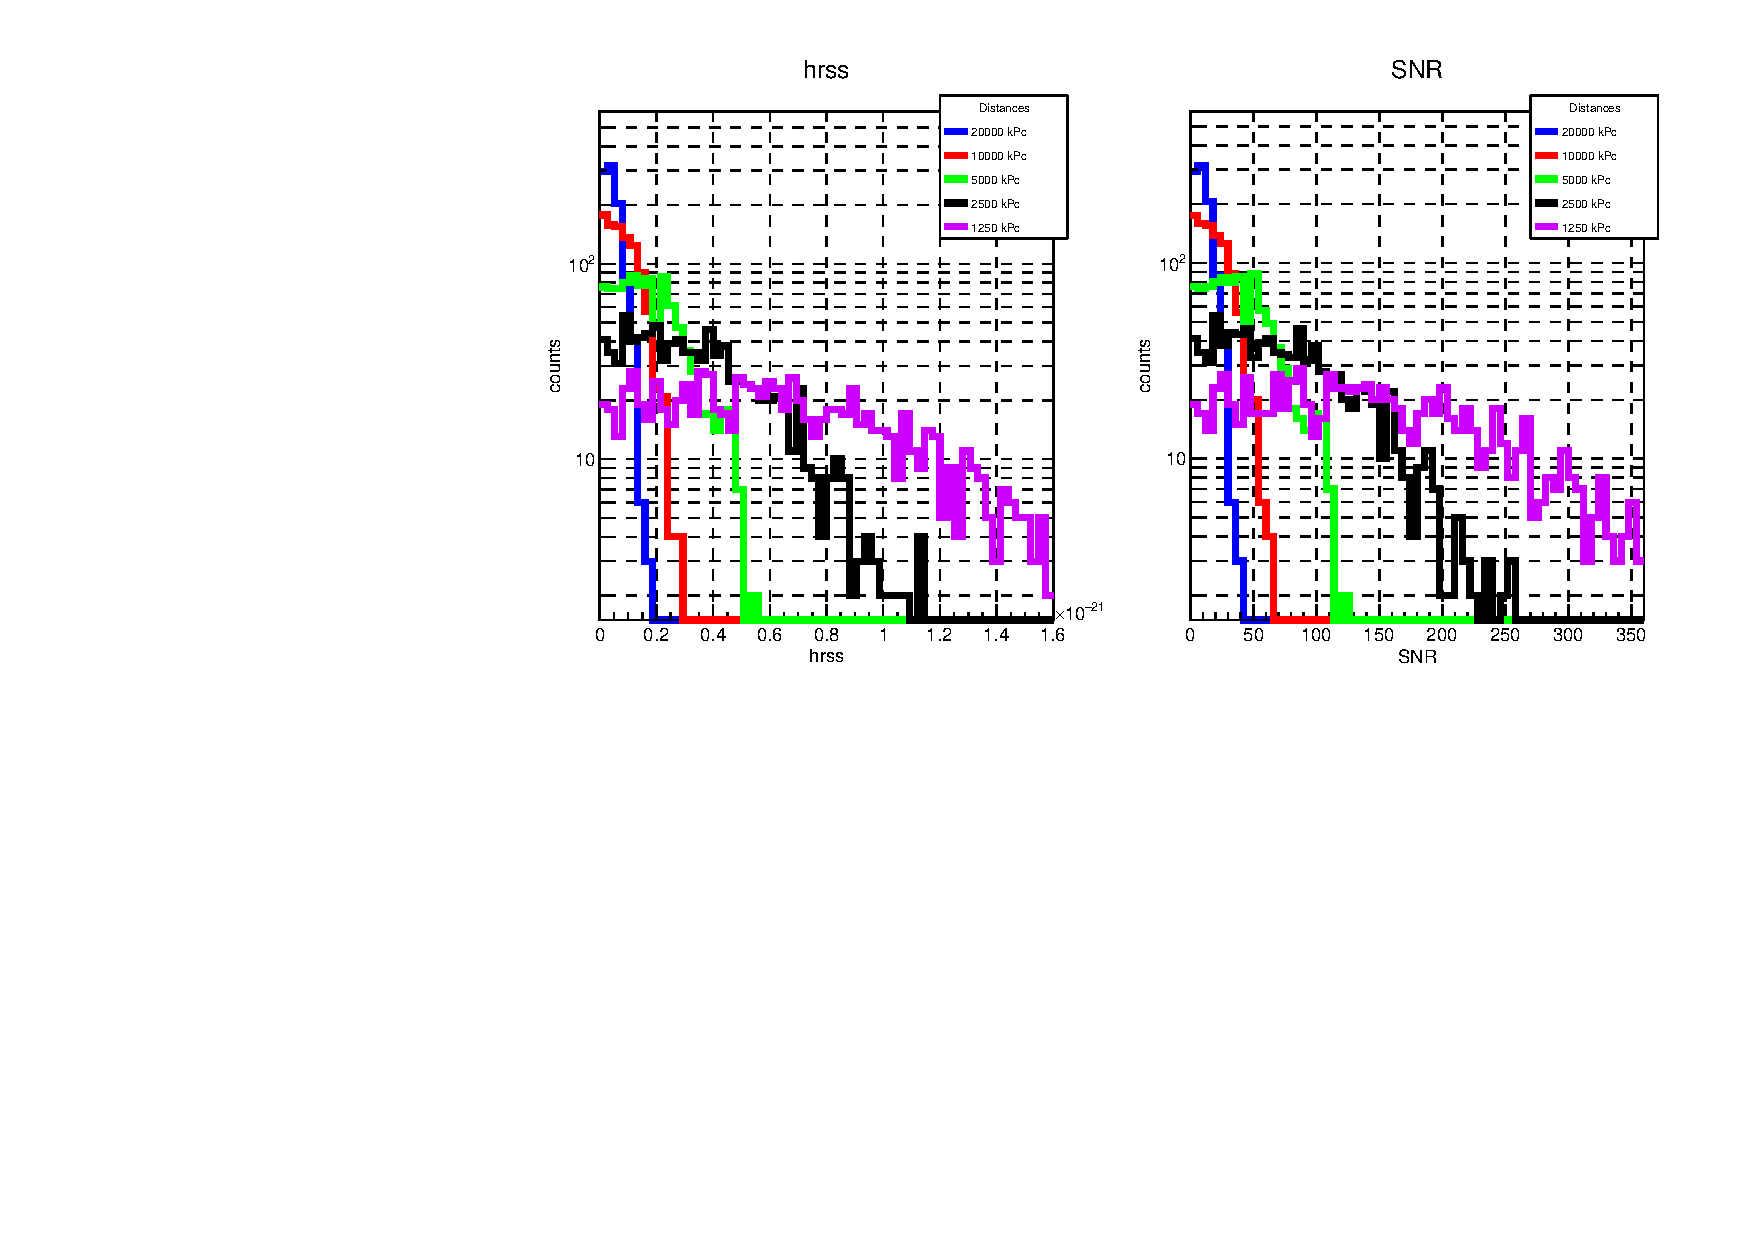
\includegraphics[scale=0.68, angle=0]{figures/Capitolo_4/hrss_snr_Distribution.pdf}
		\setlength{\belowcaptionskip}{-20pt}
		\caption{}
		\label{fig:hrss_snr_distribution}
	\end{figure}
\end{center}	

\lipsum[8]
\lipsum[9]
	% !TEX root = ./Tesi_Triennale_PMNS.tex
\chapter{Conclusioni}

\begin{center}
	$\smallsim 1/2$ pagine
\end{center}

Prova di conclusioni

\lipsum[10]

\lipsum[11]    
	
	\backmatter
	\appendix
%    \chapter{Appendice}
	\bibliographystyle{plain}
	\bibliography{BibliografiaTesi}





\end{document}
